\documentclass[10pt]{article}
\usepackage[utf8]{inputenc}
\usepackage[a4paper, portrait, margin=1in]{geometry}
\usepackage{amsmath}
\usepackage{graphicx}
\usepackage{float}
\usepackage{bytefield}


\usepackage{biblatex}
\addbibresource{ref.bib}


\title{Fantastic project}
\author{Test User}
%\date{}

% This is how you can comment in your .tex files


\begin{document}

\maketitle
\tableofcontents

\section{Introduction}

\textbf{Lorem ipsum} dolor sit amet, consectetur adipiscing elit. \textit{Quisque} at tristique sapien. Mauris ornare aliquet mauris, a elementum dui rutrum eget. Integer tellus lectus, tempor id orci id, dictum malesuada tellus. Sed lobortis id neque sit amet elementum. Suspendisse quis elementum libero. Vivamus at lobortis massa. Cras facilisis nulla odio, non efficitur arcu tempor sit amet. Proin semper convallis urna, vitae congue lorem pulvinar sed.

\section{Maths}
There is a very important theorem in maths 
$$a^2 + b^2 = c^2.$$
Another math mode example: $\frac{(1+2)*4}{2}$. \\

Now, let's create an equation:

\begin{align}
    2x + 5 &= 6\\
    2x &= 1\\
    x &= \frac{1}{2}
\end{align}

\begin{align*}
    2x + 5 &= 6\\
    2x &= 1\\
    x &= \frac{1}{2}
\end{align*}

$$\int_{a}^{b}x^2dx$$

\section{Tables}
\begin{center}
\begin{tabular}{|c|c|c|}
    \hline
    \textbf{header1} & \textbf{header2} & \textbf{header3}  \\
    \hline
    item1 & item2 & \\
    \hline
    item3 & item4 & \\
    \hline
\end{tabular}
\end{center}

\begin{center}
\begin{tabular}{||c c c c||} 
    \hline
    Col1 & Col2 & Col2 & Col3 \\ [0.5ex] 
    \hline\hline
    1 & 6 & 87837 & 787 \\ 
    \hline
    2 & 7 & 78 & 5415 \\
    \hline
    3 & 545 & 778 & 7507 \\
    \hline
    4 & 545 & 18744 & 7560 \\
    \hline
    5 & 88 & 788 & 6344 \\ [1ex] 
    \hline
\end{tabular}
\end{center}

\section{Images aka figures}
    \begin{figure}[h]
        \centering
        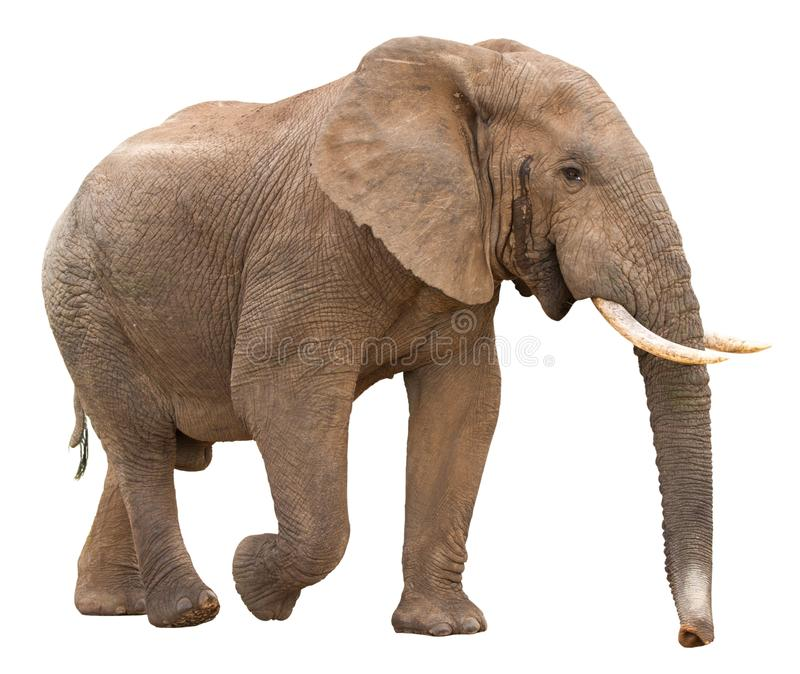
\includegraphics{elephant.jpg}
        \caption{This is an elephant!}
        \label{fig:elephant}
    \end{figure}

\section{Bytefield package experiments}
    \begin{center}
    \begin{bytefield}[bitwidth=1.0em]{40}
        \bitheader{0-39} \\
        \bitbox{4}{\textbf{type}} & \bitbox{6}{unused} & \bitbox{2}{GN} & \bitbox{10}{positionX}
        & \bitbox{10}{positionY} & \bitbox{6}{test bitbox1} & \bitbox{2}{tb2}
    \end{bytefield}
    \end{center}



\section{Main Part}
In this part there will be 3 subsections:
\begin{itemize}
    \item Subpart1
    \item Subpart2
    \item Subpart3
\end{itemize}
Enumerated version of the same list:

\begin{enumerate}
    \item Subpart1
    \item Subpart2
    \item Subpart3
\end{enumerate}



\subsection{Subpart 1}
Integer ut porta ex. Nullam bibendum erat quis massa lacinia tempus. Nam ac ultrices nulla. Praesent vel nisi tempor, feugiat magna tempus, vulputate purus. Phasellus placerat dictum dui ut pulvinar. Sed in nunc lobortis, mattis quam at, maximus tellus. Praesent erat mi, blandit in velit sed, euismod consequat diam. Praesent sit amet porta turpis. Phasellus fringilla purus sit amet metus accumsan tempus. Vivamus posuere feugiat orci, nec tristique justo congue sit amet. Sed viverra massa vel metus tempus ornare. Aliquam nulla risus, pellentesque sit amet rutrum ac, elementum non nunc. Donec lacinia dolor vel felis luctus vulputate sit amet a nisi. Vestibulum molestie aliquam lacus vitae efficitur. Aliquam quis maximus quam. Morbi hendrerit augue in nisi varius, ac mollis odio cursus. 

\subsection{Subpart 2}
In facilisis justo sed magna dignissim dignissim. Ut commodo blandit libero in fermentum. Fusce id imperdiet orci. Vestibulum dignissim nunc id tortor aliquam posuere. Vivamus rutrum magna a sem interdum dapibus at at elit. Donec tempor malesuada dui, a congue lectus vulputate at. Vestibulum sit amet vestibulum dui. Curabitur nulla odio, tincidunt viverra feugiat a, semper id ex. Duis auctor rutrum lacus sit amet semper. Integer tempus ante et ipsum tempus egestas. Sed nulla risus, varius ac euismod at, volutpat id velit. Phasellus venenatis dui ac orci mollis vulputate. Nam pulvinar odio at eros imperdiet laoreet. Nulla augue est, suscipit tempor urna quis, condimentum mattis nisi. Nam sed libero quis tortor scelerisque elementum. Morbi a orci a turpis interdum condimentum eget id metus.

\subsection{Subpart 3}
Nulla at lacus sit amet lectus consequat mollis eu sit amet est. Duis a purus enim. Suspendisse sed vestibulum lacus. Etiam ornare rhoncus lorem, ac blandit lacus condimentum sit amet. Ut sed congue massa, quis consectetur massa. Fusce tortor erat, luctus ut pretium vel, condimentum in nunc. Nulla lacinia massa ac turpis ullamcorper aliquet. Mauris eget neque congue, lacinia purus et, imperdiet nisl. Vivamus convallis posuere volutpat. Morbi sagittis felis sed est luctus congue. Duis aliquam condimentum odio, vitae bibendum orci consectetur ut. Mauris ac turpis ut neque auctor egestas. Vivamus commodo dolor in justo condimentum, nec mattis odio laoreet. Etiam id risus ante.

\section{Summary}
In this section I am referring to this fantastic article \cite{article1}.

Phasellus rhoncus leo nisl, vitae aliquet urna egestas vel. Maecenas consequat elit at enim vestibulum consectetur. Etiam varius, eros et placerat dignissim, lorem magna laoreet est, vel tincidunt sapien nibh in arcu. Nunc commodo tortor ligula, tincidunt interdum quam sagittis sed. Donec eget consectetur nunc, non elementum mi. Donec sed enim fringilla, imperdiet ligula ut, tincidunt massa. Vestibulum convallis vehicula laoreet. Duis id porttitor tellus. Quisque cursus eros id enim eleifend posuere. Sed eu molestie risus, ac sodales lectus. Duis interdum sit amet enim vitae luctus. Nunc eu cursus lacus.

\printbibliography

\end{document}